% ============================================================================
% CHƯƠNG 3: PHƯƠNG PHÁP ĐỀ XUẤT (METHODOLOGY)
% ============================================================================

\chapter{PHƯƠNG PHÁP ĐỀ XUẤT}

\section{Tổng quan Pipeline 4-Stage}

Đề tài xây dựng pipeline 4 stages để so sánh systematic giữa Weak Supervision và Supervised Learning trên gaming sentiment analysis.

\subsection{Kiến trúc Pipeline}

\begin{figure}[h]
    \centering
    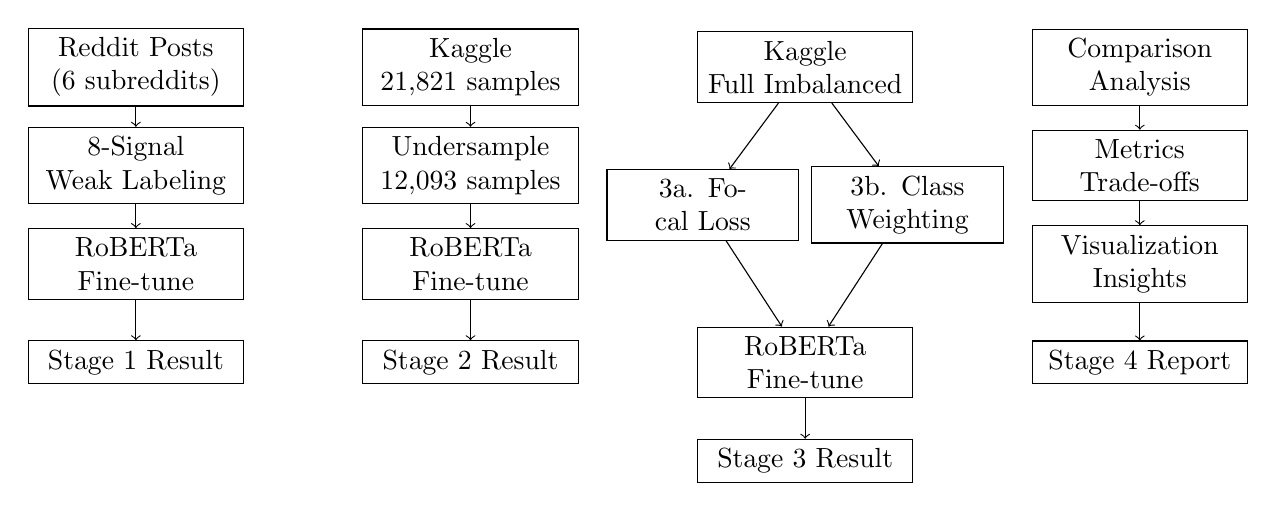
\begin{tikzpicture}[node distance=1.25cm, auto]
        % Stage 1
        \node (s1data) [rectangle, draw, text width=2.5cm, align=center] {Reddit Posts\\(6 subreddits)};
        \node (s1weak) [rectangle, draw, text width=2.5cm, align=center, below of=s1data] {8-Signal\\Weak Labeling};
        \node (s1train) [rectangle, draw, text width=2.5cm, align=center, below of=s1weak] {RoBERTa\\Fine-tune};
        \node (s1result) [rectangle, draw, text width=2.5cm, align=center, below of=s1train] {Stage 1 Result};
        
        % Stage 2
        \node (s2data) [rectangle, draw, text width=2.5cm, align=center, right of=s1data, xshift=3cm] {Kaggle\\21,821 samples};
        \node (s2balance) [rectangle, draw, text width=2.5cm, align=center, below of=s2data] {Undersample\\12,093 samples};
        \node (s2train) [rectangle, draw, text width=2.5cm, align=center, below of=s2balance] {RoBERTa\\Fine-tune};
        \node (s2result) [rectangle, draw, text width=2.5cm, align=center, below of=s2train] {Stage 2 Result};
        
        % Stage 3
        \node (s3data) [rectangle, draw, text width=2.5cm, align=center, right of=s2data, xshift=3cm] {Kaggle\\Full Imbalanced};
        % Tách nhánh Stage 3
        \node (s3a) [rectangle, draw, text width=2.2cm, align=center, below of=s3data, xshift=-1.3cm, yshift=-0.5cm] {3a. Focal Loss};
        \node (s3b) [rectangle, draw, text width=2.2cm, align=center, below of=s3data, xshift=1.3cm, yshift=-0.5cm] {3b. Class\\Weighting};
        
        \node (s3train) [rectangle, draw, text width=2.5cm, align=center, below of=s3data, yshift=-2.5cm] {RoBERTa\\Fine-tune};
        \node (s3result) [rectangle, draw, text width=2.5cm, align=center, below of=s3train] {Stage 3 Result};
        
        % Stage 4
        \node (s4compare) [rectangle, draw, text width=2.5cm, align=center, right of=s3data, xshift=3cm] {Comparison\\Analysis};
        \node (s4metrics) [rectangle, draw, text width=2.5cm, align=center, below of=s4compare] {Metrics\\Trade-offs};
        \node (s4visual) [rectangle, draw, text width=2.5cm, align=center, below of=s4metrics] {Visualization\\Insights};
        \node (s4final) [rectangle, draw, text width=2.5cm, align=center, below of=s4visual] {Stage 4 Report};
        
        % Arrows
        \draw [->] (s1data) -- (s1weak);
        \draw [->] (s1weak) -- (s1train);
        \draw [->] (s1train) -- (s1result);
        
        \draw [->] (s2data) -- (s2balance);
        \draw [->] (s2balance) -- (s2train);
        \draw [->] (s2train) -- (s2result);
        
        \draw [->] (s3data) -- (s3a);
        \draw [->] (s3data) -- (s3b);
        \draw [->] (s3a) -- (s3train);
        \draw [->] (s3b) -- (s3train);
        \draw [->] (s3train) -- (s3result);
        
        \draw [->] (s4compare) -- (s4metrics);
        \draw [->] (s4metrics) -- (s4visual);
        \draw [->] (s4visual) -- (s4final);
        

    \end{tikzpicture}
    \caption{Pipeline 4-Stage Overview}
\end{figure}


\subsection{Data Flow}

Dữ liệu đầu vào (input) cho pipeline là raw gaming text bao gồm Reddit posts và Kaggle reviews. Dữ liệu này sẽ đi qua 4 stages khác nhau, mỗi stage có phương pháp xử lý riêng biệt như mô tả dưới đây.

\subsubsection{Stage 1: Weak Supervision Flow}

\textbf{Luồng dữ liệu:} Reddit Posts $\xrightarrow{\text{8 Signals}}$ Weak Labels $\xrightarrow{\text{RoBERTa}}$ Model$_1$

\textbf{Mô tả:} Stage 1 sử dụng dữ liệu Reddit posts từ 6 subreddits gaming khác nhau. Dữ liệu này chưa có nhãn sẵn, do đó đề tài áp dụng \textbf{8-Signal Weak Labeling Strategy} để tự động gắn nhãn cho dữ liệu. 8 signals bao gồm Awards, Comments, Upvote Ratio, Score, Gaming Text Features, Sarcasm Detection, Flair Analysis, và Top Comments Sentiment. Mỗi signal sẽ vote cho một sentiment label với mức trọng số khác nhau, sau đó weighted voting mechanism kết hợp tất cả để tạo weak labels với confidence score. Chỉ những samples có confidence $\geq 0.6$ mới được giữ lại để fine-tune RoBERTa model, tạo ra Model$_1$.

\subsubsection{Stage 2: Balanced Supervised Learning Flow}

\textbf{Luồng dữ liệu:} Kaggle Reviews $\xrightarrow{\text{Undersample}}$ Balanced Data $\xrightarrow{\text{RoBERTa + CE}}$ Model$_2$

\textbf{Mô tả:} Stage 2 sử dụng Kaggle dataset với 21,821 samples đã có ground truth labels. Tuy nhiên, dataset này có class imbalance với Positive chiếm 44.8\%, Neutral 35.7\%, và Negative chỉ 18.5\%. Để tạo baseline có dữ liệu cân bằng, đề tài áp dụng \textbf{undersampling} giảm xuống còn 12,093 samples với phân bố đều giữa 3 classes. Model RoBERTa sau đó được fine-tune trên balanced data này với Cross Entropy Loss chuẩn, tạo ra Model$_2$ làm baseline để so sánh.

\subsubsection{Stage 3: Advanced Loss Functions Flow}

\textbf{Luồng dữ liệu:} Kaggle Full $\xrightarrow{\text{3a: Focal Loss} \lor \text{3b: Class Weight}}$ RoBERTa $\xrightarrow{\text{Fine-tune}}$ Model$_3$

\textbf{Mô tả:} Stage 3 sử dụng \textbf{full imbalanced Kaggle dataset} (21,821 samples) không undersample, nhằm giữ lại tất cả thông tin. Để giải quyết class imbalance, đề tài thử nghiệm 2 chiến lược algorithm-level: \textbf{Stage 3a sử dứng Focal Loss} với $\alpha=0.25, \gamma=2.0$ để down-weight easy examples và focus vào hard examples (thường là minority class); \textbf{Stage 3b sử dụng Class Weighting} với inverse frequency weighting để tăng trọng số cho minority classes trong loss function. Cả hai phương pháp đều fine-tune RoBERTa trên full data, tạo ra Model$_{3a}$ và Model$_{3b}$ tương ứng.

\subsubsection{Stage 4: Comparative Analysis Flow}

\textbf{Luồng dữ liệu:} (Model$_1$, Model$_2$, Model$_3$) $\xrightarrow{\text{Evaluation}}$ Trade-off Analysis

\textbf{Mô tả:} Stage 4 không train model mới, mà thực hiện \textbf{comprehensive evaluation và comparison} giữa tất cả các models từ 3 stages trước. Evaluation bao gồm các metrics như Accuracy, Precision, Recall, F1-Score (macro và weighted), Confusion Matrix. Ngoài ra, stage này còn phân tích trade-offs giữa các phương pháp: Weak Supervision (chất lượng nhãn noisy nhưng không cần labeling cost), Balanced data (mất dữ liệu nhưng đơn giản), Focal Loss (phức tạp hơn nhưng hiệu quả với imbalance), và Class Weighting (đơn giản nhưng hiệu quả). Kết quả cuối cùng là báo cáo chi tiết về insights, recommendations, và visualizations để giúp hiểu rõ ưu nhược điểm của từng approach.

% ----------------------------------------------------------------------------
\section{Stage 1: Weak Supervision với 8-Signal Strategy}

\subsection{Kiến trúc OptimizedWeakLabelGenerator}

\begin{figure}[h]
    \centering
    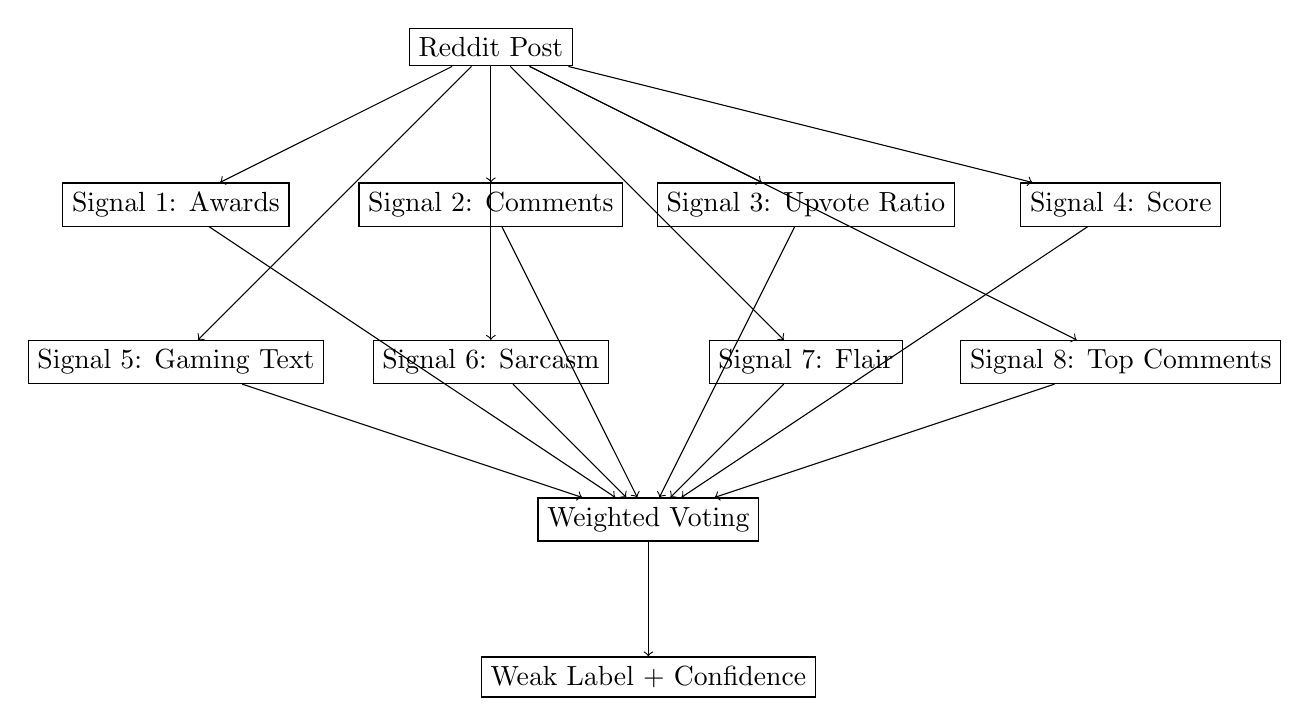
\begin{tikzpicture}[node distance=2cm, auto]
        \node (input) [rectangle, draw] {Reddit Post};
        \node (s1) [rectangle, draw, below of=input, xshift=-4cm] {Signal 1: Awards};
        \node (s2) [rectangle, draw, right of=s1, xshift=2cm] {Signal 2: Comments};
        \node (s3) [rectangle, draw, right of=s2, xshift=2cm] {Signal 3: Upvote Ratio};
        \node (s4) [rectangle, draw, right of=s3, xshift=2cm] {Signal 4: Score};
        \node (s5) [rectangle, draw, below of=s1] {Signal 5: Gaming Text};
        \node (s6) [rectangle, draw, right of=s5, xshift=2cm] {Signal 6: Sarcasm};
        \node (s7) [rectangle, draw, right of=s6, xshift=2cm] {Signal 7: Flair};
        \node (s8) [rectangle, draw, right of=s7, xshift=2cm] {Signal 8: Top Comments};
        \node (vote) [rectangle, draw, below of=s6, xshift=2cm] {Weighted Voting};
        \node (output) [rectangle, draw, below of=vote] {Weak Label + Confidence};
        
        \draw [->] (input) -- (s1);
        \draw [->] (input) -- (s2);
        \draw [->] (input) -- (s3);
        \draw [->] (input) -- (s4);
        \draw [->] (input) -- (s5);
        \draw [->] (input) -- (s6);
        \draw [->] (input) -- (s7);
        \draw [->] (input) -- (s8);
        \draw [->] (s1) -- (vote);
        \draw [->] (s2) -- (vote);
        \draw [->] (s3) -- (vote);
        \draw [->] (s4) -- (vote);
        \draw [->] (s5) -- (vote);
        \draw [->] (s6) -- (vote);
        \draw [->] (s7) -- (vote);
        \draw [->] (s8) -- (vote);
        \draw [->] (vote) -- (output);
    \end{tikzpicture}
    \caption{OptimizedWeakLabelGenerator Architecture}
\end{figure}

\subsection{Chi tiết 8 Signals với Trọng số}

\subsubsection{Signal 1: Awards Analysis (Weight: 4.0)}

Reddit awards (Gold, Silver, Platinum) là tín hiệu premium nhất vì require chi phí thực từ users. Khác với upvotes (free), việc trao awards thể hiện sự \textbf{highly engaged và genuine appreciation} từ cộng đồng. Một post nhận nhiều awards thường mang nội dung chất lượng cao, hữu ích, hoặc rất positive (ví dụ: game review xuất sắc, gameplay highlights, helpful guides). Do vậy, signal này được gán \textbf{trọng số cao nhất (4.0)} trong 8 signals vì độ tin cậy cao và noise thấp.

\textbf{Logic và Implementation:}

\begin{minted}[linenos, breaklines, frame=single, fontsize=\small]{python}
def analyze_awards(post):
    """
    Phân tích số lượng awards của post để đánh giá sentiment.
    
    Args:
        post: Reddit post object chứa thông tin total_awards_received
    
    Returns:
        tuple: (sentiment_label, weight)
            - 'positive' với weight 4.0 nếu total_awards >= 5 (strongly positive)
            - 'positive' với weight 3.5 nếu total_awards >= 2 (moderately positive)
            - (None, 0) nếu không đủ điều kiện (abstain)
    """
    total_awards = post.total_awards_received
    
    if total_awards >= 5:
        return ('positive', 4.0)  # Strongly positive - exceptional content
    elif total_awards >= 2:
        return ('positive', 3.5)  # Moderately positive - good content
    else:
        return (None, 0)  # Abstain - not enough signal
\end{minted}

\textbf{Giải thích chi tiết:} Nếu post có $\geq 5$ awards, đây là exceptional content với strongly positive sentiment (weight 4.0 tối đa). Nếu $\geq 2$ awards, đây là good content với moderately positive sentiment (weight 3.5). Nếu $< 2$ awards, signal này không đủ mạnh để kết luận, do đó abstain (không vote). Lý do trọng số cao nhất: awards cần chi phí thực (tiền) nên là high-quality signal với ít noise, khác với upvotes có thể bị manipulate dễ dàng.

\subsubsection{Signal 2: Comments Count (Weight: 3.0)}

Số lượng comments phản ánh mức độ \textbf{engagement và discussion intensity} của cộng đồng. Posts với nhiều comments thường là nội dung gây chú ý, thú vị, hoặc controversial. Trong gaming context, high engagement thường liên quan đến positive content (exciting news, impressive gameplay) hoặc heated discussions. Moderate comments (50-100) thường là discussions trung lập, trong khi very low comments (<3) với positive score biểu thị low engagement neutral content.

\textbf{Logic với dynamic weighting:}

\begin{minted}[linenos, breaklines, frame=single, fontsize=\small]{python}
def analyze_comments(post):
    """
    Phân tích số lượng comments để đánh giá engagement và sentiment.
    
    Args:
        post: Reddit post object chứa num_comments và score
    
    Returns:
        tuple: (sentiment_label, weight) dựa trên số comments và score
    """
    num_comments = post.num_comments
    score = post.score
    
    if num_comments > 200:
        # Very high engagement - usually positive viral content
        return ('positive', 3.0)
    elif num_comments > 100:
        # High engagement - likely positive or interesting
        return ('positive', 2.5)
    elif 50 <= num_comments <= 100:
        # Moderate discussion - neutral content
        return ('neutral', 2.0)
    elif num_comments < 3 and score > 0:
        # Low engagement but positive score - likely neutral
        return ('neutral', 1.0)
    else:
        # Not enough signal to determine
        return (None, 0)
\end{minted}

\textbf{Giải thích chi tiết:} Signal này sử dụng \textbf{dynamic weighting} dựa trên mức độ engagement. Posts có $>200$ comments thường là viral positive content (exciting game releases, amazing updates) với weight 3.0. Posts có $>100$ comments vẫn là highly engaging content với weight 2.5. Khoảng 50-100 comments biểu thị moderate discussion (neutral) với weight 2.0. Very low engagement ($<3$ comments nhưng positive score) thường là neutral content ít tranh cãi với weight 1.0. Trọng số cao (3.0 max) vì engagement là tín hiệu mạnh về community interest.

\subsubsection{Signal 3: Upvote Ratio (Weight: 2.5)}

Upvote ratio phản ánh \textbf{community consensus} về một post. Nó được tính bằng tỷ lệ giữa upvotes và tổng số votes, cho biết % users đồng tình với nội dung. Ratio cao ($\geq 0.95$) biểu thị overwhelming support (strongly positive content), ratio thấp ($< 0.45$) biểu thị strong disagreement (negative content), và ratio trung bình ($0.55-0.70$) biểu thị controversial/divisive content (neutral hoặc mixed opinions).

\textbf{Công thức:}
\begin{equation}
    \text{Upvote Ratio} = \frac{\text{upvotes}}{\text{upvotes} + \text{downvotes}}
\end{equation}

\textbf{Threshold Analysis và Giải thích:} Upvote ratio $\geq 0.95$ biểu thị overwhelming positive consensus (95\% users đồng ý) với weight 2.5 - thường là universally praised content. Ratio $\geq 0.85$ là strong positive (85\% support) với weight 2.2 - content chất lượng cao. Khoảng $0.55 - 0.70$ biểu thị controversial/divisive content với neutral label và weight 2.0 - opinions rất mixed, không rõ ràng positive hay negative. Cuối cùng, $< 0.45$ biểu thị negative consensus (majority disagrees) với weight 2.5 - thường là complaints, rants, hoặc unpopular opinions. Trọng số 2.5 cao vì upvote ratio là direct measure của community sentiment, không bị bias bởi số lượng votes (khác với score).

\subsubsection{Signal 4: Post Score (Weight: 2.0)}

Post score được tính bằng upvotes - downvotes, là \textbf{net popularity indicator} của post. Khác với upvote ratio (tỷ lệ consensus), score phản ánh \textbf{số lượng tuyệt đối} users upvote. Score cao ($>500$) biểu thị viral positive content với wide reach, score trung bình ($>100$) là popular positive content, score gần 0 ($0-10$) là low engagement neutral, và negative score ($<-10$) biểu thị strongly disliked content. Signal này có weight trung bình (2.0) vì có thể bị skew bởi timing và subreddit size.

\textbf{Logic và Implementation:}

\begin{minted}[linenos, breaklines, frame=single, fontsize=\small]{python}
def analyze_score(post):
    """
    Phân tích post score (net upvotes) để đánh giá popularity và sentiment.
    
    Args:
        post: Reddit post object chứa score (upvotes - downvotes)
    
    Returns:
        tuple: (sentiment_label, weight) dựa trên score thresholds
    """
    score = post.score
    
    if score > 500:
        # Viral content - very high positive engagement
        return ('positive', 2.0)
    elif score > 100:
        # Popular content - good positive reception
        return ('positive', 1.8)
    elif 0 <= score <= 10:
        # Low engagement - likely neutral
        return ('neutral', 1.8)
    elif score < -10:
        # Heavily downvoted - strongly negative
        return ('negative', 2.0)
    else:
        # Ambiguous range (score between -10 and 0)
        return (None, 0)
\end{minted}

\textbf{Giải thích chi tiết:} Score $>500$ biểu thị viral positive content với weight 2.0 - đây là posts được cộng đồng rất yêu thích. Score $>100$ là popular positive content với weight 1.8 - tốt nhưng chưa viral. Score trong khoảng $0-10$ biểu thị low engagement neutral với weight 1.8 - không gây tranh cãi. Score $<-10$ là strongly negative với weight 2.0 - bị community reject mạnh. Trọng số 2.0 trung bình vì score có thể bị ảnh hưởng bởi factors khác (posting time, subreddit size, visibility), không chỉ sentiment.

\subsubsection{Signal 5: Gaming Text Features (Weight: 1.8-3.0)}

Signal này phân tích \textbf{gaming-specific vocabulary} trong text để detect sentiment. Gaming community có ngôn ngữ riêng biệt với slang, jargon, và các terms đặc thù không có trong general sentiment lexicons. Đề tài design \textbf{3-tier weighting system} dựa trên strength của sentiment indicators: Strong indicators (weight 3.0) là các terms cực kỳ mạnh (GOTY, masterpiece, unplayable), N-grams (weight 2.5) là các phrases phức tạp (worth the price, waste of money), và Single keywords (weight 1.8-2.2) là các từ đơn (amazing, buggy). Trọng số cao (tới 3.0) vì gaming vocabulary là \textbf{domain-specific strong signal} rất reliable trong gaming context.

\textbf{Gaming Lexicon:}

\begin{table}[h]
    \centering
    \caption{Gaming-Specific Vocabulary (50+ terms)}
    \begin{tabular}{|l|l|l|}
        \hline
        \textbf{Tier} & \textbf{Positive Terms} & \textbf{Negative Terms} \\
        \hline
        Strong (3.0) & masterpiece, GOTY, flawless & unplayable, broken mess, cash grab \\
        \hline
        N-grams (2.5) & worth the price, must play & waste of money, avoid this \\
        \hline
        Keywords (1.8) & amazing, addictive, polished & buggy, p2w, grindy, laggy \\
        \hline
    \end{tabular}
\end{table}

\textbf{Implementation với 3-Tier System:}

\begin{minted}[linenos, breaklines, frame=single, fontsize=\small]{python}
def extract_gaming_text_features(text):
    """
    Phân tích gaming-specific vocabulary trong text để detect sentiment.
    Sử dụng 3-tier weighting: Strong (3.0), N-grams (2.5), Keywords (1.8-2.2).
    
    Args:
        text: String chứa post title và content
    
    Returns:
        tuple: (sentiment_label, weight) dựa trên strongest gaming term found
    """
    text_lower = text.lower()
    
    # Tier 1: Strong indicators (weight 3.0) - cực kỳ mạnh
    strong_pos = ['masterpiece', 'goty', 'game of the year', 'flawless',
                  'perfect game', 'instant classic']
    strong_neg = ['unplayable', 'broken mess', 'cash grab', 'scam',
                  'worst game', 'complete failure']
    
    for term in strong_pos:
        if term in text_lower:
            return ('positive', 3.0)  # Strongest positive signal
    for term in strong_neg:
        if term in text_lower:
            return ('negative', 3.0)  # Strongest negative signal
    
    # Tier 2: N-grams/Phrases (weight 2.5) - phrases phức tạp
    ngram_pos = ['worth the price', 'must play', 'highly recommend',
                 'best game', 'absolutely love']
    ngram_neg = ['waste of money', 'avoid this', "don't buy",
                 'not worth it', 'save your money']
    
    for term in ngram_pos:
        if term in text_lower:
            return ('positive', 2.5)  # Strong positive phrase
    for term in ngram_neg:
        if term in text_lower:
            return ('negative', 2.5)  # Strong negative phrase
    
    # Tier 3: Single keywords (weight 1.8-2.2) - đếm số lượng keywords
    pos_count = count_positive_keywords(text_lower)
    neg_count = count_negative_keywords(text_lower)
    
    if pos_count >= 2:
        # Multiple positive keywords - quite positive
        return ('positive', 2.2)
    elif neg_count >= 2:
        # Multiple negative keywords - quite negative
        return ('negative', 2.2)
    elif pos_count == 1:
        # Single positive keyword - moderately positive
        return ('positive', 1.8)
    elif neg_count == 1:
        # Single negative keyword - moderately negative
        return ('negative', 1.8)
    
    # No gaming keywords found
    return (None, 0)
\end{minted}

\textbf{Giải thích chi tiết:} Hàm kiểm tra text theo thứ tự \textbf{từ mạnh đến yếu}. Đầu tiên kiểm tra Strong indicators (tier 1) với weight 3.0 - các terms cực kỳ mạnh như "GOTY" (Game of the Year), "masterpiece", "unplayable". Nếu không tìm thấy, kiểm tra N-grams (tier 2) với weight 2.5 - các phrases phức tạp như "worth the price", "waste of money". Cuối cùng đếm Single keywords (tier 3) với weight 1.8-2.2 tùy số lượng. System này đảm bảo strongest signal được ưu tiên, và weight cao hơn cho multiple occurrences.

\subsubsection{Signal 6: Sarcasm Detection (Flip Sentiment)}

Sarcasm là một \textbf{thách thức lớn} trong sentiment analysis, đặc biệt trong gaming community nơi users thường dùng sarcasm để biểu thị thất vọng. Ví dụ: "Yeah, 60 FPS on a 4090, totally optimized /s" - literal sentiment là positive ("totally optimized") nhưng thực tế là negative sarcasm. Signal này không gán weight trực tiếp mà \textbf{flip sentiment} (positive $\leftrightarrow$ negative) khi detect sarcasm markers. Đây là \textbf{modifier signal} quan trọng để correct false positives/negatives.

\textbf{Patterns:} Có 2 loại patterns: \textbf{explicit sarcasm} với "/s" tag rõ ràng (Reddit convention), và \textbf{implicit sarcasm} với các phrases như "yeah right", "totally", "sure", "perfectly" kết hợp với negative context.

\textbf{Logic và Implementation:}

\begin{minted}[linenos, breaklines, frame=single, fontsize=\small]{python}
def detect_sarcasm(text):
    """
    Detect sarcasm markers trong text.
    
    Args:
        text: String chứa post title và content
    
    Returns:
        bool: True nếu detect sarcasm, False nếu không
    """
    # List of sarcasm markers (both explicit and implicit)
    sarcasm_markers = [
        '/s',                    # Explicit Reddit sarcasm tag
        'yeah right',            # Implicit sarcasm phrase
        'totally balanced',      # Gaming sarcasm (unbalanced mechanics)
        'perfectly optimized',   # Gaming sarcasm (poor optimization)
        'great job /s',          # Explicit negative sarcasm
        'well done /s',          # Explicit negative sarcasm
        'amazing work /s'        # Explicit negative sarcasm
    ]
    
    text_lower = text.lower()
    for marker in sarcasm_markers:
        if marker in text_lower:
            return True  # Sarcasm detected
    return False  # No sarcasm

# Usage in main labeling function:
if detect_sarcasm(text):
    # Flip sentiment: positive <-> negative (neutral unchanged)
    if predicted_label == 'positive':
        predicted_label = 'negative'
    elif predicted_label == 'negative':
        predicted_label = 'positive'
    # Note: neutral remains neutral (no flip needed)
\end{minted}

\textbf{Giải thích chi tiết:} Hàm kiểm tra danh sách sarcasm markers trong text. Nếu detect được bất kỳ marker nào, hàm trả về True. Trong main labeling logic, nếu detect sarcasm, sentiment label sẽ \textbf{bị flip}: positive $\rightarrow$ negative và ngược lại (neutral không flip). Ví dụ: nếu text "This game is great /s" ban đầu được label positive (do từ "great"), sau khi detect "/s" sẽ flip thành negative (thể hiện thực tế là game tệ). Signal này rất quan trọng để handle gaming community's sarcastic tone.

\subsubsection{Signal 7: Flair Analysis (Weight: 2.0-3.5)}

Reddit flairs là \textbf{user-assigned categories} cho posts, thường rất reliable vì users tự chọn flair phù hợp với nội dung. Flairs như "Rant", "Bug", "Complaint" chỉ rõ negative sentiment, trong khi "Praise", "Recommendation" chỉ positive sentiment. "Discussion", "Question" thường neutral. Signal này có \textbf{weight rất cao (2.0-3.5)} vì flair là explicit intent signal từ chính user, không cần inference. Ví dụ: post với flair "Rant" chắc chắn là negative (weight 3.5), "Praise" chắc chắn positive (weight 3.5).

\textbf{Flair Mapping và Implementation:}

\begin{minted}[linenos, breaklines, frame=single, fontsize=\small]{python}
def analyze_flair(post):
    """
    Phân tích Reddit post flair để determine sentiment.
    
    Args:
        post: Reddit post object chứa link_flair_text
    
    Returns:
        tuple: (sentiment_label, weight) dựa trên flair mapping
    """
    # Flair-to-sentiment mapping với weights
    flair_mapping = {
        # Negative flairs (high weight - strong signal)
        'Rant': ('negative', 3.5),        # Chắc chắn negative
        'Bug': ('negative', 3.0),         # Technical issues
        'Complaint': ('negative', 3.0),   # User complaints
        'Issue': ('negative', 2.5),       # Problems/issues
        
        # Positive flairs (high weight - strong signal)
        'Praise': ('positive', 3.5),      # Chắc chắn positive
        'Recommendation': ('positive', 3.0), # Recommend game
        'Review': ('positive', 2.5),      # Usually positive reviews
        
        # Neutral flairs (medium weight)
        'Discussion': ('neutral', 2.0),   # General discussion
        'Question': ('neutral', 2.0),     # Asking questions
        'Help': ('neutral', 2.0)          # Seeking help
    }
    
    flair = post.link_flair_text
    if flair and flair in flair_mapping:
        return flair_mapping[flair]  # Return (label, weight)
    else:
        return (None, 0)  # No flair or unknown flair
\end{minted}

\textbf{Giải thích chi tiết:} Hàm kiểm tra post flair và map với sentiment label tương ứng. \textbf{Negative flairs} (Rant, Bug, Complaint) có weight cao nhất 3.0-3.5 vì rõ ràng biểu thị user dissatisfaction. \textbf{Positive flairs} (Praise, Recommendation) cũng có weight 2.5-3.5 biểu thị satisfaction. \textbf{Neutral flairs} (Discussion, Question, Help) có weight trung bình 2.0. Nếu post không có flair hoặc flair unknown, signal abstain. Flair là một trong những signals reliable nhất vì đến từ user's explicit categorization.

\subsubsection{Signal 8: Top Comments Sentiment (Weight: 2.0-2.5)}

Top comments phản ánh \textbf{community response} và discussion tone xung quanh post. Nếu top comments positive (agree, praise, support), post thường positive. Nếu top comments negative (criticize, disagree, complaints), post thường negative. Signal này analyze \textbf{top 3 comments} (highest score) vì đây là community consensus - top comments được upvoted nhiều nhất biểu thị majority opinion. Weight 2.0-2.5 vì comments có thể không relate trực tiếp đến post sentiment, nhưng vẫn là useful signal.

\textbf{Logic và Implementation:}

\begin{minted}[linenos, breaklines, frame=single, fontsize=\small]{python}
def analyze_top_comments(post):
    """
    Phân tích top 3 comments để capture community response sentiment.
    
    Args:
        post: Reddit post object để lấy comments
    
    Returns:
        tuple: (sentiment_label, weight) dựa trên comments sentiment
    """
    # Lấy top 3 comments (sorted by score)
    top_comments = get_top_comments(post, limit=3)
    
    pos_count = 0  # Count positive comments
    neg_count = 0  # Count negative comments
    
    for comment in top_comments:
        # Check sentiment of each comment
        if contains_positive_words(comment.body):
            # Weighted by comment score (higher score = stronger signal)
            pos_count += (1 if comment.score < 50 else 1.2)
        elif contains_negative_words(comment.body):
            neg_count += (1 if comment.score < 50 else 1.2)
    
    # Determine sentiment based on counts
    if pos_count >= 2:
        # Strong positive response (2+ positive comments)
        return ('positive', 2.5)
    elif neg_count >= 2:
        # Strong negative response (2+ negative comments)
        return ('negative', 2.5)
    elif pos_count > neg_count:
        # Moderate positive response
        return ('positive', 2.0)
    elif neg_count > pos_count:
        # Moderate negative response
        return ('negative', 2.0)
    else:
        # Mixed or neutral response
        return ('neutral', 2.0)
\end{minted}

\textbf{Giải thích chi tiết:} Hàm lấy top 3 comments (highest scores) và kiểm tra sentiment của mỗi comment. Mỗi comment được \textbf{weighted by score}: comments với score $\geq 50$ (highly upvoted) nhận multiplier 1.2, comments score $< 50$ nhận 1.0. Nếu có $\geq 2$ positive comments, trả về positive với weight 2.5 (strong positive response). Tương tự cho negative. Nếu \texttt{pos\_count} $>$ \texttt{neg\_count} (nhưng chưa đạt 2), trả về positive với weight 2.0 (moderate). Nếu bằng nhau hoặc không rõ ràng, trả về neutral với weight 2.0. Signal này capture \textbf{community consensus} thông qua top-voted comments.

\subsection{Weighted Voting Mechanism}

\subsubsection{Công thức Voting}

Aggregate 8 signals với trọng số để tạo final label:

\begin{equation}
    \text{Score}(c) = \sum_{i=1}^{8} w_i \cdot \mathbb{1}(\text{Signal}_i = c)
\end{equation}

\begin{equation}
    \text{Label}_{\text{pred}} = \arg\max_{c \in \{P, N, Ne\}} \text{Score}(c)
\end{equation}

\textbf{Confidence Scoring:}
\begin{equation}
    \text{Confidence} = \frac{\text{Score}(\text{Label}_{\text{pred}})}{\sum_{i=1}^{8} w_i}
\end{equation}

với threshold: $\text{Confidence} \geq 0.6$

\subsubsection{Implementation}

\begin{minted}[linenos, breaklines, frame=single, fontsize=\small]{python}
def generate_optimized_weak_label(post):
    """
    Tạo weak label cho Reddit post bằng weighted voting từ 8 signals.
    
    Args:
        post: Reddit post object
    
    Returns:
        tuple: (predicted_label, confidence) hoặc (None, confidence) nếu low confidence
    """
    signals = []
    
    # Collect all 8 signals
    signals.append(analyze_awards(post))              # Signal 1: Awards (weight 4.0)
    signals.append(analyze_comments(post))            # Signal 2: Comments (weight 3.0)
    signals.append(analyze_upvote_ratio(post))        # Signal 3: Upvote Ratio (weight 2.5)
    signals.append(analyze_score(post))               # Signal 4: Score (weight 2.0)
    signals.append(extract_gaming_text_features(post))# Signal 5: Gaming Text (weight 1.8-3.0)
    signals.append(analyze_flair(post))               # Signal 7: Flair (weight 2.0-3.5)
    signals.append(analyze_top_comments(post))        # Signal 8: Top Comments (weight 2.0-2.5)
    
    # Weighted voting
    votes = {'positive': 0, 'negative': 0, 'neutral': 0}
    total_weight = 0
    
    for label, weight in signals:
        if label is not None:
            votes[label] += weight
            total_weight += weight
    
    # Get winner (label with highest weighted votes)
    predicted_label = max(votes, key=votes.get)
    confidence = votes[predicted_label] / total_weight if total_weight > 0 else 0
    
    # Signal 6: Sarcasm detection (flip sentiment if sarcasm detected)
    text = post.title + ' ' + post.selftext
    if detect_sarcasm(text):
        if predicted_label == 'positive':
            predicted_label = 'negative'
        elif predicted_label == 'negative':
            predicted_label = 'positive'
        # Note: neutral remains unchanged
    
    # Check confidence threshold (only keep high-confidence labels)
    if confidence >= 0.6:
        return predicted_label, confidence  # High confidence - accept label
    else:
        return None, confidence  # Low confidence - reject sample
\end{minted}


% ----------------------------------------------------------------------------
\section{Stage 2 – Supervised Learning (Balanced)}

Giai đoạn 2 tập trung xây dựng một mô hình baseline nhằm đánh giá năng lực của RoBERTa trên dữ liệu đã được cân bằng lớp. Mục tiêu là loại bỏ \textit{data bias} từ sự mất cân bằng dữ liệu và cung cấp điểm chuẩn để so sánh với các chiến lược nâng cao (Class Weighting, Focal Loss) trong Giai đoạn 3.

\subsection{Chiến lược Cân bằng Dữ liệu: Undersampling}

Dữ liệu gốc của bộ review game mất cân bằng rõ rệt, với lớp \textit{Positive} chiếm đa số trong khi \textit{Neutral} và \textit{Negative} ít mẫu hơn. Điều này làm tăng nguy cơ mô hình thiên vị lớp đa số, dẫn đến giảm Recall và F1 của các lớp thiểu số, đặc biệt đối với các bình luận tiêu cực. Để khắc phục, chiến lược \textbf{Undersampling} được áp dụng, nhằm cân bằng số lượng mẫu giữa các lớp trước khi huấn luyện mà không cần thay đổi hàm mất mát.  

Đầu tiên xác định số lượng mẫu tối thiểu $n_{\min}$ trong tập huấn luyện:

\[
n_{\min} = \min_{c \in C} (N_c)
\]

trong đó $N_c$ là số mẫu của lớp $c$. Sau đó, mỗi lớp được randomly sampled về $n_{\min}$ mẫu:

\[
\text{balanced\_train\_val} = \bigcup_{c \in C} \text{RandomSample}(D_c, n_{\min})
\]

Chiến lược này giúp mô hình học đồng đều các đặc trưng của lớp thiểu số, giữ gradient ổn định trong quá trình huấn luyện và không làm mất thông tin quan trọng từ lớp đa số. 

\begin{minted}[linenos, breaklines, frame=single, fontsize=\small]{python}
class_counts = train_val_df[label_col].value_counts()
min_count = class_counts.min()

balanced_train_val_df = train_val_df.groupby(label_col).apply(
    lambda x: x.sample(min_count, random_state=42)
).reset_index(drop=True)
\end{minted}

Sau khi cân bằng, dữ liệu được chia Train/Validation theo tỉ lệ 80/20 bằng \textit{stratified split} để duy trì cân bằng lớp, trong khi Test Set vẫn giữ nguyên phân phối gốc, giúp đánh giá mô hình một cách công bằng:

\begin{minted}[linenos, breaklines, frame=single, fontsize=\small]{python}
train_df, val_df = train_test_split(
    balanced_train_val_df,
    test_size=0.2,
    stratify=balanced_train_val_df[label_col],
    random_state=42
)
\end{minted}

Chiến lược Undersampling là một \textit{data-level approach} đơn giản nhưng hiệu quả, giúp mô hình học đồng đều đặc trưng của lớp thiểu số mà không làm mất thông tin lớp đa số, đồng thời cung cấp baseline rõ ràng để so sánh với các chiến lược nâng cao như Class Weighting hoặc Focal Loss trong Stage 3.

\subsection{Tiền xử lý và Cấu hình Huấn luyện}

\textbf{Tokenization và Ánh xạ Nhãn:} 
\begin{itemize}
    \item \textbf{Tokenizer}: AutoTokenizer từ \texttt{cardiffnlp/twitter-roberta-base-sentiment-latest}.
    \item \textbf{Encoding}: \texttt{truncation=True}, \texttt{padding="max\_length"}, \texttt{max\_length=512} để giữ toàn bộ thông tin bình luận dài.
    \item \textbf{Ánh xạ nhãn}: \texttt{label2id}, dữ liệu được chuyển sang HF Dataset để tối ưu tải GPU.
\end{itemize}

\begin{minted}[linenos, breaklines, frame=single, fontsize=\small]{python}
tokenizer = AutoTokenizer.from_pretrained(MODEL)

def tokenize(example):
    return tokenizer(example["text"], truncation=True, padding="max_length", max_length=512)
\end{minted}

\noindent $\Rightarrow$ Tokenization chuẩn hóa văn bản, giúp mô hình học chính xác các đặc trưng ngôn ngữ, kể cả slang và emoji phổ biến trong bình luận game.

\textbf{Hàm compute\_metrics:} 


Hàm này tính các chỉ số \textit{accuracy}, \textit{F1-weighted} và \textit{F1-macro} nhằm đánh giá hiệu năng phân loại một cách toàn diện. F1-weighted phản ánh hiệu năng tổng thể, cân nhắc số lượng mẫu từng lớp, trong khi F1-macro đánh giá đồng đều giữa tất cả các lớp, đặc biệt quan trọng khi dữ liệu mất cân bằng và dùng để so sánh với các chiến lược nâng cao. Hàm được truyền vào Trainer qua tham số \texttt{compute\_metrics}, đảm bảo mỗi lần đánh giá trên tập validation hoặc test trả về đầy đủ bộ metric, hỗ trợ tối ưu hóa mô hình.

\begin{minted}[linenos, breaklines, frame=single, fontsize=\small]{python}
def compute_metrics(p):
    predictions = np.argmax(p.predictions, axis=1)
    labels = p.label_ids
    acc = accuracy_score(labels, predictions)
    f1_weighted = f1_score(labels, predictions, average='weighted')
    f1_macro = f1_score(labels, predictions, average='macro')
    return {
        'accuracy': acc,
        'f1_weighted': f1_weighted,
        'f1_macro': f1_macro
    }
\end{minted}

\textbf{Tham số Huấn luyện và Loss Function}

Mô hình RoBERTa được fine-tune trên dữ liệu cân bằng sử dụng \texttt{CrossEntropyLoss}, do Undersampling đã cân bằng số lượng mẫu, nên không cần weighted loss. Các tham số huấn luyện được cấu hình qua \texttt{TrainingArguments} như sau:

\begin{minted}[linenos, breaklines, frame=single, fontsize=\small]{python}
training_args = TrainingArguments(
    output_dir="./stage2_roberta_balanced_final",
    num_train_epochs=3,
    per_device_train_batch_size=16,
    per_device_eval_batch_size=32,
    learning_rate=2e-5,
    weight_decay=0.05,
    warmup_steps=500,
    eval_strategy="steps",
    eval_steps=200,
    load_best_model_at_end=True,
    metric_for_best_model="f1",
    max_grad_norm=1.0
)
\end{minted}

\textbf{Phân tích:}
\begin{itemize}
    \item \textbf{Learning rate = 2e-5}: giữ nguyên kiến thức tiền huấn luyện, tránh làm mất embedding đã học.
    \item \textbf{Weight decay = 0.05}: thực hiện regularization, giúp hạn chế overfitting trên tập nhỏ sau undersampling.
    \item \textbf{Batch size = 16 (Train) / 32 (Eval)}: cân bằng giữa tốc độ huấn luyện và ổn định gradient.
    \item \textbf{Max gradient norm = 1.0}: áp dụng gradient clipping, tránh hiện tượng exploding gradient.
    \item \textbf{Metric F1-weighted}: đánh giá hiệu quả mô hình đồng đều trên các lớp, đặc biệt quan trọng với lớp thiểu số.
    \item \textbf{Warmup steps = 500}: giúp ổn định quá trình huấn luyện ban đầu, tránh sốc gradient.
\end{itemize}
\textbf{Trainer}


Khởi tạo Trainer kết hợp mô hình, dataset, tokenizer, data collator, callback và hàm metrics.

\begin{minted}[linenos, breaklines, frame=single, fontsize=\small]{python}
trainer = Trainer(
    model=model,  # RoBERTa model
    args=training_args,  # training arguments
    train_dataset=train_data,  # training dataset
    eval_dataset=val_data,  # validation dataset
    tokenizer=tokenizer,  # tokenizer cho padding/encoding
    data_collator=DataCollatorWithPadding(tokenizer),  # dynamic padding
    callbacks=[EarlyStoppingCallback(early_stopping_patience=2)],  # early stopping
    compute_metrics=compute_metrics  # hàm tính accuracy, F1-weighted, F1-macro
)
\end{minted}

Trainer tích hợp toàn bộ pipeline huấn luyện của Hugging Face, trong đó \texttt{data\_collator} đảm bảo mỗi batch được padding động để tối ưu hiệu năng GPU. Đồng thời, \texttt{EarlyStoppingCallback} sẽ dừng quá trình huấn luyện nếu kết quả trên tập validation không cải thiện liên tiếp 2 lần, giúp tránh overfitting và tiết kiệm thời gian. Hàm \texttt{compute\_metrics} được sử dụng để trả về các chỉ số \textit{accuracy}, \textit{F1-weighted} (phản ánh hiệu năng tổng thể) và \textit{F1-macro} (đánh giá đồng đều tất cả các lớp, đặc biệt quan trọng với dữ liệu mất cân bằng).

% ----------------------------------------------------------------------------

\section{Stage 3a: Focal Loss}
\subsection{Chiến lược: Focal Loss}

Để giải quyết vấn đề mất cân bằng dữ liệu nghiêm trọng trong tập dữ liệu Kaggle, đề tài áp dụng chiến lược Focal Loss thay vì Cross Entropy truyền thống.

\subsubsection{Công thức toán học}

Focal Loss được định nghĩa như sau:

\begin{equation}
    FL(p_t) = -\alpha_t (1 - p_t)^{\gamma} \log(p_t)
\end{equation}

Trong đó, $p_t$ là xác suất dự đoán đúng của mô hình đối với nhãn thực tế (ground truth); $\alpha_t$ (alpha) là tham số cân bằng (balancing factor) giúp điều chỉnh trọng số giữa các lớp positive/negative; $\gamma$ (gamma) là tham số tập trung (focusing parameter) giúp điều chỉnh mức độ giảm trọng số của các mẫu dễ; và $(1 - p_t)^{\gamma}$ là hệ số điều chỉnh (modulating factor).

\subsubsection{Cơ chế hoạt động và Ý nghĩa}

Focal Loss hoạt động dựa trên 3 cơ chế chính. \textbf{Thứ nhất, giảm trọng số mẫu dễ (Down-weighting easy examples):} Khi một mẫu được phân loại đúng với độ tự tin cao ($p_t \to 1$), hệ số $(1 - p_t)^{\gamma}$ sẽ tiến về 0, làm cho đóng góp của mẫu đó vào tổng loss trở nên rất nhỏ, giúp mô hình không bị chi phối bởi số lượng lớn các mẫu dễ (thường thuộc lớp đa số như Positive). \textbf{Thứ hai, tập trung vào mẫu khó (Focusing on hard examples):} Khi một mẫu bị phân loại sai hoặc độ tự tin thấp ($p_t \to 0$), hệ số $(1 - p_t)^{\gamma}$ sẽ gần bằng 1, lúc này Focal Loss xấp xỉ Cross Entropy Loss và giữ nguyên mức độ phạt lớn đối với mô hình, nhờ đó quá trình huấn luyện sẽ tập trung cập nhật trọng số để cải thiện khả năng nhận diện các mẫu khó (thường thuộc lớp thiểu số như Negative). \textbf{Thứ ba, cân bằng lớp (Class Balancing):} Tham số $\alpha_t$ được thiết lập khác nhau cho từng lớp để bù đắp sự chênh lệch số lượng mẫu, tương tự như phương pháp Class Weighting nhưng được tích hợp trực tiếp vào hàm loss.


\subsection{FocalLoss Class Design}

Class FocalLoss kế thừa từ \texttt{torch.nn.Module} và implement Focal Loss formula. Class này nhận 3 parameters: \texttt{alpha} (balancing factor, default 0.25), \texttt{gamma} (focusing parameter, default 2.0), và \texttt{num\_classes} (số classes, default 3 cho sentiment). Method \texttt{forward()} thực hiện 7 steps: compute probabilities qua softmax, one-hot encode labels, lấy $p_t$ (probability for true class), tính focal weight $(1-p_t)^\gamma$, tính cross entropy loss, kết hợp với alpha và focal weight, và return mean loss.

\begin{minted}[linenos, breaklines, frame=single, fontsize=\small]{python}
import torch
import torch.nn as nn
import torch.nn.functional as F

class FocalLoss(nn.Module):
    """
    Focal Loss for addressing class imbalance.
    
    FL(p_t) = -alpha_t * (1 - p_t)^gamma * log(p_t)
    
    Args:
        alpha (float): Balancing factor for class weighting
        gamma (float): Focusing parameter for hard examples
        num_classes (int): Number of output classes
    """
    
    def __init__(self, alpha=0.25, gamma=2.0, num_classes=3):
        super(FocalLoss, self).__init__()
        self.alpha = alpha
        self.gamma = gamma
        self.num_classes = num_classes
    
    def forward(self, logits, labels):
        """
        Args:
            logits: (batch_size, num_classes) - Raw model outputs
            labels: (batch_size,) - Ground truth class indices
        
        Returns:
            loss: Scalar focal loss value
        """
        # Step 1: Compute probabilities via softmax
        probs = F.softmax(logits, dim=-1)  # (batch, num_classes)
        
        # Step 2: One-hot encode labels
        labels_one_hot = F.one_hot(labels, self.num_classes).float()
        
        # Step 3: Get p_t (probability for true class)
        p_t = (probs * labels_one_hot).sum(dim=1)  # (batch,)
        
        # Step 4: Compute focal weight: (1 - p_t)^gamma
        focal_weight = (1 - p_t) ** self.gamma
        
        # Step 5: Compute cross entropy loss
        ce_loss = F.cross_entropy(logits, labels, reduction='none')
        
        # Step 6: Combine with alpha and focal weight
        focal_loss = self.alpha * focal_weight * ce_loss
        
        # Step 7: Return mean loss
        return focal_loss.mean()
\end{minted}

\subsection{FocalLossTrainer}

\texttt{FocalLossTrainer} là custom Trainer kế thừa từ Hugging Face \texttt{Trainer} class, override method \texttt{compute\_loss()} để sử dụng Focal Loss thay vì Cross Entropy Loss mặc định. Trong \texttt{\_\_init\_\_()} method, FocalLoss object được khởi tạo với \texttt{alpha} và \texttt{gamma} parameters. Method \texttt{compute\_loss()} thực hiện forward pass qua model, lấy logits, rồi tính Focal Loss với labels. Đây là cách tiêu chuẩn để integrate custom loss function với Hugging Face training pipeline.

\begin{minted}[linenos, breaklines, frame=single, fontsize=\small]{python}
from transformers import Trainer

class FocalLossTrainer(Trainer):
    """
    Custom Trainer using Focal Loss instead of CrossEntropyLoss.
    """
    
    def __init__(self, *args, alpha=0.25, gamma=2.0, **kwargs):
        super().__init__(*args, **kwargs)
        self.focal_loss = FocalLoss(
            alpha=alpha, 
            gamma=gamma, 
            num_classes=3
        )
    
    def compute_loss(self, model, inputs, return_outputs=False):
        """
        Override compute_loss to use Focal Loss.
        """
        labels = inputs.pop("labels")
        
        # Forward pass
        outputs = model(**inputs)
        logits = outputs.logits
        
        # Compute focal loss
        loss = self.focal_loss(logits, labels)
        
        return (loss, outputs) if return_outputs else loss
\end{minted}

\subsection{Training Configuration}

Training configuration được thiết lập qua \texttt{TrainingArguments} của Hugging Face. Các hyperparameters quan trọng bao gồm: 
\path{num_train_epochs=3}, 
\path{per_device_train_batch_size=16} và 
\path{eval_batch_size=32}, 
\path{learning_rate=2e-5} với 
\path{weight_decay=0.01} cho optimizer, 
\path{warmup_steps=500} để tăng dần learning rate, 
\path{evaluation_strategy='epoch'} để evaluate mỗi epoch, 
\path{load_best_model_at_end=True} để giữ model tốt nhất, 
\path{metric_for_best_model='eval_accuracy'}, và 
\path{fp16=True} để enable mixed precision training (giảm memory, tăng tốc độ).

\begin{minted}[linenos, breaklines, frame=single, fontsize=\small]{python}
from transformers import TrainingArguments

training_args = TrainingArguments(
    output_dir='./results_stage3_focal',
    
    # Training parameters
    num_train_epochs=3,
    per_device_train_batch_size=16,
    per_device_eval_batch_size=32,
    
    # Optimizer
    learning_rate=2e-5,
    weight_decay=0.01,
    warmup_steps=500,
    
    # Evaluation
    evaluation_strategy='epoch',
    save_strategy='epoch',
    load_best_model_at_end=True,
    metric_for_best_model='eval_accuracy',
    
    # Logging
    logging_steps=100,
    logging_dir='./logs_stage3',
    
    # Hardware
    fp16=True,  # Mixed precision training
)
\end{minted}


\subsection{Training Process}

Quá trình training bao gồm 3 bước chính. \textbf{Bước 1:} Initialize RoBERTa model từ pre-trained checkpoint \texttt{cardiffnlp/twitter-roberta-base-sentiment-latest} với \texttt{num\_labels=3} cho 3-class sentiment. \textbf{Bước 2:} Khởi tạo \texttt{FocalLossTrainer} với model, training arguments, datasets, và Focal Loss parameters (\texttt{alpha=0.25, gamma=2.0}). \textbf{Bước 3:} Gọi \texttt{trainer.train()} để bắt đầu training, sau đó \texttt{trainer.evaluate()} để đánh giá performance trên validation set. Kết quả bao gồm accuracy và F1-score.

\begin{minted}[linenos, breaklines, frame=single, fontsize=\small]{python}
# Initialize model
from transformers import AutoModelForSequenceClassification

model = AutoModelForSequenceClassification.from_pretrained(
    'cardiffnlp/twitter-roberta-base-sentiment-latest',
    num_labels=3,
    ignore_mismatched_sizes=True
)

# Initialize trainer with Focal Loss
trainer = FocalLossTrainer(
    model=model,
    args=training_args,
    train_dataset=train_dataset,
    eval_dataset=val_dataset,
    alpha=0.25,  # Focal Loss alpha
    gamma=2.0,   # Focal Loss gamma
    compute_metrics=compute_metrics
)

# Train
trainer.train()

# Evaluate
results = trainer.evaluate()
print(f"Accuracy: {results['eval_accuracy']:.4f}")
print(f"F1-Score: {results['eval_f1']:.4f}")
\end{minted}


% ----------------------------------------------------------------------------


\section{Stage 3b: Class Weighting}
\subsection{Chiến lược Class Weighting}

Dữ liệu cảm xúc về game thường mất cân bằng, với lớp Positive chiếm đa số, trong khi Negative và Neutral ít mẫu hơn. Điều này khiến mô hình dễ thiên về lớp đa số, giảm hiệu quả nhận diện các lớp ít xuất hiện – đặc biệt là những bình luận tiêu cực quan trọng trong đánh giá game.

Chiến lược \textbf{Class Weighting} giải quyết vấn đề này bằng cách tác động trực tiếp vào hàm mất mát (Loss Function): các lớp thiểu số được tăng trọng số, giúp mô hình học đồng đều trên tất cả các lớp mà không cần thay đổi dữ liệu. Kết hợp với tiêu chí F1-macro, chiến lược này cân bằng giữa độ chính xác tổng thể và khả năng nhận diện lớp thiểu số, phù hợp với dataset gaming reviews có nhiều slang và ngôn ngữ đặc thù.
\subsubsection{Cơ sở Toán học và Tính toán Trọng số}

Chúng em sử dụng \textbf{Tần suất Nghịch đảo có điều chỉnh Logarit} (Log-scaled Inverse Frequency Weighting) để giảm trọng số quá lớn cho lớp cực thiểu và giữ quá trình huấn luyện ổn định.

\textbf{Tính Trọng số Nghịch đảo Logarit}

\[
w'_j = \frac{1}{\ln(1+n_j)}
\]

\begin{itemize}
    \item $n_j$: số lượng mẫu thuộc lớp $j$ trong tập huấn luyện.
    \item Logarit giúp giảm chênh lệch quá lớn giữa lớp đa số (Positive) và lớp thiểu số (Negative).
\end{itemize}

\textbf{Chuẩn hóa Trọng số}

\[
w_j = \frac{w'_j}{\sum_{k=1}^{K} w'_k}, \quad K=3 \text{ (Negative, Neutral, Positive)}
\]

Chuẩn hóa đảm bảo tổng trọng số bằng 1, giữ tỷ lệ ảnh hưởng hợp lý giữa các lớp.

\textbf{Code tính trọng số lớp}
\begin{minted}[linenos, breaklines, frame=single, fontsize=\small]{python}
# 1. Lấy số lượng mẫu huấn luyện của từng lớp
train_counts = train_df["label_id"].value_counts().sort_index()

# 2. Tính trọng số nghịch đảo logarit
weights = 1 / np.log1p(train_counts)

# 3. Chuẩn hóa trọng số
weights = weights / weights.sum()

# 4. Chuyển sang PyTorch Tensor và đưa lên GPU
class_weights = torch.tensor(weights.values, dtype=torch.float32).to(device)
\end{minted}


\textbf{Phân tích:} Trọng số lớn hơn dành cho lớp ít mẫu, nhỏ hơn cho lớp đa số nhưng không quá cực đoan nhờ logarit. Điều này giữ gradient ổn định khi backpropagation, tránh mô hình bị “quá nhạy” với các mẫu hiếm. Đây là một cách tiếp cận thuật toán-level, không thay đổi dữ liệu, giữ nguyên toàn bộ thông tin từ tập huấn luyện.

\subsubsection{Tích hợp vào Hàm Mất mát (Weighted Cross-Entropy Loss)}

\[
\text{Loss} = -\frac{1}{N} \sum_{i=1}^{N} w_{y_i} \log(p_{i, y_i})
\]

\begin{itemize}
    \item $w_{y_i}$: trọng số lớp của nhãn thực tế $y_i$.
    \item $p_{i, y_i}$: xác suất dự đoán cho lớp $y_i$ của mẫu thứ $i$.
\end{itemize}

\textbf{Cơ chế hoạt động}

\begin{itemize}
    \item Khi một mẫu thuộc lớp thiểu số bị phân loại sai, gradient được nhân với trọng số lớn hơn → tăng cường điều chỉnh các tham số của mô hình cho lớp này.
    \item Mẫu lớp đa số bị sai vẫn có gradient, nhưng trọng số nhỏ hơn → giảm tác động thiên lệch về lớp đa số.
    \item Kết quả: RoBERTa học đồng đều trên tất cả lớp, cải thiện recall/F1-score cho Negative và Neutral mà không ảnh hưởng nhiều đến Positive.
\end{itemize}

\textbf{Code triển khai WeightedCELoss}
\begin{minted}[frame=single, fontsize=\small, linenos, breaklines]{python}
class WeightedCELoss(nn.Module):
    def __init__(self, weights):
        super().__init__()
        self.weights = weights  # Tensor [w_0, w_1, w_2]

    def forward(self, logits, labels):
        return F.cross_entropy(logits, labels, weight=self.weights)

ce_loss_fn = WeightedCELoss(class_weights)
\end{minted}

\textbf{Phân tích chi tiết}

Cross-Entropy Loss chuẩn: mỗi lỗi mẫu đều ảnh hưởng bằng 1. WeightedCE: nhấn mạnh lỗi của lớp ít mẫu, giảm lỗi lớp nhiều mẫu.

Trong backpropagation:

\[
\frac{\partial \text{Loss}}{\partial z_j} = w_{y_i} (p_j - y_j)
\]

\noindent $\Rightarrow$ Gradient được scale theo trọng số lớp, giúp optimizer điều chỉnh weights của mô hình tập trung hơn vào lớp thiểu số. Chiến lược này đơn giản, dễ triển khai, phù hợp với các dataset gaming reviews mất cân bằng mà vẫn giữ thông tin lớp đa số.So với Cross-Entropy chuẩn, WeightedCE nhấn mạnh lớp ít mẫu, giữ gradient ổn định, cải thiện recall và F1 cho các lớp ít mẫu (Negative/Neutral) mà không làm giảm hiệu năng lớp đa số (Positive).

\subsection{Tiền xử lí và Cấu hình Huấn luyện}
\subsubsection{Tiền xử lí}
\textbf{Phân chia Dữ liệu}

Dữ liệu được chia thành Train, Validation và Test với tỉ lệ 70/15/15, sử dụng \textit{stratified split} để đảm bảo cân bằng tỉ lệ lớp trong từng split. Việc này giúp giữ nguyên phân phối lớp và minh họa trực quan sự cân bằng dữ liệu.

\begin{minted}[frame=single, fontsize=\small, linenos, breaklines]{python}
# Chia Train/Validation/Test
train_df, temp_df = train_test_split(
    df, test_size=0.3, stratify=df['label_id'], random_state=42
)

val_df, test_df = train_test_split(
    temp_df, test_size=0.5, stratify=temp_df['label_id'], random_state=42
)
\end{minted}

\textbf{Tokenization và ánh xạ nhãn}\\
Tokenization được thực hiện bằng \texttt{AutoTokenizer} từ mô hình, với truncation và padding \texttt{"max \_length"}, giữ toàn bộ thông tin từ các bình luận dài. Nhãn được ánh xạ sang dạng số (\texttt{label2id}) để phù hợp với mô hình và HF Dataset.

\begin{minted}[frame=single, fontsize=\small, linenos, breaklines]{python}
tokenizer = AutoTokenizer.from_pretrained(MODEL_NAME)

def tokenize_fn(examples):
    return tokenizer(examples[text_col], truncation=True, padding=True, max_length=512)

# Chuyển DataFrame → HF Dataset
train_ds = Dataset.from_pandas(train_df[[text_col, 'label_id']].rename(columns={'label_id': 'label'}))
val_ds   = Dataset.from_pandas(val_df[[text_col, 'label_id']].rename(columns={'label_id': 'label'}))
test_ds  = Dataset.from_pandas(test_df[[text_col, 'label_id']].rename(columns={'label_id': 'label'}))
\end{minted}

\subsubsection{Cấu hình Huấn luyện}\\
\textbf{Weighted Loss và Custom Trainer}
Để sử dụng hàm mất mát \texttt{WeightedCELoss} trong framework Hugging Face Trainer, chúng em tạo lớp \texttt{WeightedTrainer} kế thừa từ \texttt{Trainer} và ghi đè phương thức \texttt{compute\_loss()}. Cơ chế này cho phép mô hình RoBERTa sử dụng trực tiếp trọng số lớp khi tính loss, từ đó học đồng đều trên cả lớp đa số và lớp thiểu số.

\begin{minted}[frame=single, fontsize=\small, linenos, breaklines]{python}
class WeightedTrainer(Trainer):
    def __init__(self, loss_fn, *args, **kwargs):
        super().__init__(*args, **kwargs)
        self.loss_fn = loss_fn

    def compute_loss(self, model, inputs, return_outputs=False, **kwargs):
        labels = inputs.pop("labels")
        outputs = model(**inputs)
        loss = self.loss_fn(outputs.logits, labels)
        return (loss, outputs) if return_outputs else loss
\end{minted}

 \textbf{Cấu hình TrainingArguments}:

\begin{minted}[frame=single, fontsize=\small, linenos, breaklines]{python}
training_args = TrainingArguments(
    output_dir="./stage3_roberta_class_weight",  # checkpoint folder
    num_train_epochs=5,
    per_device_train_batch_size=16,
    per_device_eval_batch_size=32,
    warmup_steps=500,                            # LR warmup
    learning_rate=1e-5,                          # base LR
    weight_decay=0.01,
    eval_strategy="steps",
    eval_steps=200,
    load_best_model_at_end=True,                 # restore best checkpoint
    metric_for_best_model="f1_macro",
    max_grad_norm=1.0                            # gradient clipping
)
)
\end{minted}

Các tham số huấn luyện được lựa chọn nhằm đảm bảo quá trình fine-tuning mô hình RoBERTa ổn định và hiệu quả khi áp dụng weighted loss. Learning rate thấp (1e-5) giúp tránh hiện tượng gradient overshoot, đặc biệt khi lớp thiểu số được scale trọng số lên, từ đó giảm rủi ro dao động lớn của loss. Warmup steps 500 cho phép tăng dần learning rate từ 0 đến giá trị gốc trong giai đoạn đầu huấn luyện, giúp tránh sốc gradient và cải thiện sự ổn định, nhất là với tập dữ liệu nhỏ hoặc mất cân bằng. Weight decay 0.01 thực hiện L2 regularization, hạn chế overfitting và tránh mô hình trở nên quá nhạy với các lớp ít mẫu. Kích thước batch được cân đối giữa train và eval nhằm tối ưu tốc độ huấn luyện đồng thời giữ gradient ổn định, giúp optimizer cập nhật weights hiệu quả và tận dụng GPU tốt hơn. Việc đánh giá trên tập validation theo mỗi 200 bước kết hợp với \texttt{load\_best\_model\_at\_end} đảm bảo lưu lại mô hình tốt nhất dựa trên metric \texttt{f1\_macro}, từ đó tránh mất hiệu năng do dao động của loss trong huấn luyện. Metric \texttt{f1\_macro} được ưu tiên nhằm tối ưu đồng đều trên tất cả các lớp, cải thiện recall và F1 cho các lớp thiểu số mà vẫn giữ hiệu năng lớp đa số. Cuối cùng, \texttt{max\_grad\_norm = 1.0} thực hiện gradient clipping, giúp ổn định quá trình backpropagation và tránh exploding gradient, đặc biệt khi gradient của các lớp ít mẫu bị scale lên nhờ weighted loss.


\textbf{WeightedTrainer}


Khởi tạo Trainer kết hợp mô hình, dataset, tokenizer, data collator, callback và hàm loss:

\begin{minted}[frame=single, fontsize=\small, linenos, breaklines]{python}
trainer = WeightedTrainer(
    loss_fn=ce_loss_fn,                                           # weighted loss
    model=model,                                                  # RoBERTa model
    args=training_args,                                           # training arguments
    train_dataset=train_ds,                                       # training dataset
    eval_dataset=val_ds,                                          # validation dataset
    tokenizer=tokenizer,                                          # tokenizer for padding/encoding
    data_collator=DataCollatorWithPadding(tokenizer),             # dynamic padding
    callbacks=[EarlyStoppingCallback(early_stopping_patience=3)], # early stopping
    compute_metrics=compute_metrics                               # metric function
)
\end{minted}

WeightedTrainer tích hợp mô hình RoBERTa với hàm loss đã cân lớp (weighted loss), giúp gradient của các lớp ít mẫu được tăng cường, từ đó cải thiện khả năng nhận diện lớp thiểu số mà vẫn giữ thông tin lớp đa số. DataCollatorWithPadding đảm bảo mỗi batch được padding động, tối ưu bộ nhớ GPU và tốc độ huấn luyện. EarlyStoppingCallback với \texttt{patience=3} dừng huấn luyện khi \texttt{f1\_macro} trên validation không cải thiện sau 3 lần đánh giá liên tiếp, tránh overfitting. Hàm \texttt{compute\_metrics} theo dõi \texttt{f1\_macro}, \texttt{f1\_weighted} và \texttt{accuracy}, cung cấp đánh giá đồng đều giữa các lớp và giám sát hiệu năng mô hình xuyên suốt quá trình huấn luyện.

Như vậy, với chiến lược này, mô hình RoBERTa học đồng đều trên các lớp, cải thiện recall/F1 cho Negative và Neutral, đồng thời giữ hiệu năng lớp Positive. Weighted Cross-Entropy nhấn mạnh lớp ít mẫu nhưng vẫn đảm bảo gradient ổn định, giúp huấn luyện hiệu quả, đơn giản và dễ triển khai.

% ----------------------------------------------------------------------------
\section{Evaluation Metrics}

\subsection{Metrics cho Multi-class Classification}

\subsubsection{Accuracy}

Tỷ lệ phân loại đúng tổng thể:

\begin{equation}
    \text{Accuracy} = \frac{\text{TP} + \text{TN}}{\text{Total Samples}} = \frac{\sum_{i=1}^{N} \mathbb{1}(y_i = \hat{y}_i)}{N}
\end{equation}

\textbf{Ưu điểm:} Đơn giản, dễ hiểu

\textbf{Nhược điểm:} Misleading với imbalanced data (high accuracy nhưng poor minority class)

\subsubsection{Precision, Recall, F1-Score}

\textbf{Precision (Độ chính xác):} Tỷ lệ dự đoán đúng trong các predictions positive

\begin{equation}
    \text{Precision}_c = \frac{\text{TP}_c}{\text{TP}_c + \text{FP}_c}
\end{equation}

\textbf{Recall (Độ phủ):} Tỷ lệ phát hiện đúng trong tất cả mẫu positive thực tế

\begin{equation}
    \text{Recall}_c = \frac{\text{TP}_c}{\text{TP}_c + \text{FN}_c}
\end{equation}

\textbf{F1-Score:} Harmonic mean của Precision và Recall

\begin{equation}
    \text{F1}_c = 2 \cdot \frac{\text{Precision}_c \cdot \text{Recall}_c}{\text{Precision}_c + \text{Recall}_c}
\end{equation}

\subsubsection{Macro vs Weighted F1}

\textbf{F1-Macro:} Trung bình không trọng số (tất cả classes đều quan trọng)

\begin{equation}
    \text{F1-Macro} = \frac{1}{K} \sum_{c=1}^{K} \text{F1}_c
\end{equation}

\textbf{F1-Weighted:} Trung bình có trọng số theo kích thước class

\begin{equation}
    \text{F1-Weighted} = \sum_{c=1}^{K} \frac{n_c}{N} \cdot \text{F1}_c
\end{equation}

với $n_c$ là số mẫu class $c$, $N$ là tổng số mẫu.

\textbf{Khi nào dùng:}
\begin{itemize}
    \item F1-Macro: Quan tâm đều tất cả classes (including minority)
    \item F1-Weighted: Phản ánh hiệu suất tổng thể (majority class matter more)
\end{itemize}

\subsection{Confusion Matrix}

\textbf{Định nghĩa:} Ma trận $C \in \mathbb{R}^{K \times K}$ với $C_{ij}$ = số mẫu true class $i$ được predict là class $j$.

\begin{equation}
    C = \begin{bmatrix}
    \text{TP}_{\text{Neg}} & \text{FP}_{\text{Neu (from Neg)}} & \text{FP}_{\text{Pos (from Neg)}} \\
    \text{FP}_{\text{Neg (from Neu)}} & \text{TP}_{\text{Neu}} & \text{FP}_{\text{Pos (from Neu)}} \\
    \text{FP}_{\text{Neg (from Pos)}} & \text{FP}_{\text{Neu (from Pos)}} & \text{TP}_{\text{Pos}}
    \end{bmatrix}
\end{equation}

\textbf{Ví dụ Stage 3 Confusion Matrix (normalized):}

\begin{table}[h]
    \centering
    \caption{Confusion Matrix (Stage 3 Focal Loss)}
    \begin{tabular}{|l|c|c|c|}
        \hline
        \textbf{True / Pred} & \textbf{Negative} & \textbf{Neutral} & \textbf{Positive} \\
        \hline
        Negative & 0.85 & 0.10 & 0.05 \\
        \hline
        Neutral & 0.08 & 0.88 & 0.04 \\
        \hline
        Positive & 0.03 & 0.07 & 0.90 \\
        \hline
    \end{tabular}
\end{table}

\textbf{Phân tích:}
\begin{itemize}
    \item Diagonal cao (0.85, 0.88, 0.90) = good classification
    \item Main confusion: Negative $\leftrightarrow$ Neutral (0.10, 0.08)
    \item Ít confusion Negative $\leftrightarrow$ Positive (0.05, 0.03) = the model distinguishes the extremes well
\end{itemize}



% ----------------------------------------------------------------------------
% End of Chapter 3
% ----------------------------------------------------------------------------
